\documentclass[8pt, table, xcdraw]{article}%
\usepackage[a4paper, top=1cm, bottom=4cm, left=2cm, right=2cm]{geometry}%
\usepackage{amsfonts}
\usepackage{fancyhdr}
\usepackage{comment}
\usepackage{times}
\usepackage{xcolor}
\usepackage{tikz}
\usepackage{float}
\usepackage{amsmath}
\usepackage{changepage}
\usepackage{amssymb}
\usepackage{graphicx}
\usepackage{parskip}
\usepackage{listings}
\usepackage{enumerate}
\usepackage{enumitem}
\usepackage{siunitx}
\usepackage{hyperref}
\usepackage[bottom]{footmisc}
\usepackage[T1]{fontenc}
\usepackage[export]{adjustbox}
\usepackage{multirow}
\usepackage{siunitx}
\usepackage{subcaption}
\usepackage{epsfig}
\usepackage[normalem]{ulem}
\useunder{\uline}{\ul}{}
\usepackage[utf8]{inputenc}

\lstset{
 %frame=tb, % for the lines above and under the code snippets
 language=C,
 aboveskip=3mm,
 belowskip=3mm,
 showstringspaces=false,
 columns=flexible,
 basicstyle={\footnotesize\ttfamily},
 numbers=none,
 numberstyle=\tiny\color{gray},
 keywordstyle=\color{blue},
 commentstyle=\color{gray},
 stringstyle=\color{purple},
 breaklines=true,
 breakatwhitespace=true,
 literate={_}{\textunderscore}1 {([a-z])([A-Z])}{{\1}\allowbreak{\2}}{1},
 tabsize=3,
 escapeinside={/*!}{!*/},
 escapebegin=\color{black}
}

\title{
\textit{Short Circuit}\\
\vspace{15px}
\huge
C++\\
\vspace{20px}
\large
A Tour of C++\\
by Bjarne Stroustrup\\
Second Edition\\
\textcolor{gray}{Up until Section 13.3}
}
\author{Summary by Emiel Bos}
\date{}

\begin{document}

\maketitle

\section{Basics}

Source files have to be processed by a compiler, producing object files, which are combined by a linker yielding an executable program for a specific hardware/system combination.\\
When we talk about portability of C++ programs, we usually mean portability of source code.\\
The C++ standard library is implemented in C++ itself (with very minor uses of machine code for things such as thread context switching).\\
C++ is a statically typed language; the type of every entity (e.g., object, value, name, and expression) must be known to the compiler at its point of use.

\subsection{Programs}

\subsubsection{Minimal program}
\lstinline|int main() { }| is the minimal program.
The \lstinline{int} return value indicates success (\lstinline{0}) or failure (nonzero) to the system. Windows-based environments rarely make use of this value, but Linux/Unix-based environments do.

One way to minimize surprises from uncaught exceptions is to use a \lstinline{main()} with a \lstinline{try}-block as its body.

\subsubsection{Statement groups}
\lstinline|{ }| groups statements in C++.

\subsubsection{Namespaces}
A declarative region that provides a scope to the identifiers inside it and a method for preventing name conflicts in large projects. Works with block like \lstinline|namespace name { }|. All blocks of the same name are in the same scope. \lstinline{using namespace std;} makes names from \lstinline{std} visible without \lstinline{std::}.

\subsubsection{Resource} \label{resource}
Anything that has to be acquired and (explicitly or implicitly) released after use. Examples are memory, locks, sockets, file handles, and thread handles.

\subsubsection{Static allocation} \label{staticallocation}
The memory for your variables is allocated when the program starts. The size is fixed when the program is created. It applies to \hyperref[globalscope]{global} variables, file scope variables, and \lstinline{static} variables defined inside functions.

\subsubsection{Automatic allocation} \label{automaticallocation}
The memory for (non-\lstinline{static}) variables inside functions is allocated automatically on the \textit{stack}. In practice, you don't have to reserve extra memory using them, but you have limited control over the \hyperref[localscope]{lifetime} of this memory.

\subsubsection{Dynamic allocation} \label{dynamicallocation}
The memory for variables initialized with \hyperref[new]{\lstinline{new}} is allocated on the \textit{heap}/\textit{free store}. In practice, you now control the exact size and the lifetime of these memory locations, which comes with the responsibility of deallocating the memory, or you'll get memory leaks (which may lead to crashes when memory is depleted).

\subsection{Types, variables and operators}

\subsubsection{Type}
Defines a set of possible values and a set of operations (for an object).

\subsubsection{Object}
Some memory that holds a value of some type

\subsubsection{Value}
A set of bits interpreted according to a type.

\subsubsection{Variable}
A named object.

\subsubsection{\lstinline{sizeof()}}
The size of a type is implementation-defined and can be obtained by the \lstinline{sizeof(type)} operator as the number of bytes. Typical sizes are listed.

\subsubsection{Fundamental types and literals}

\begin{itemize}[leftmargin=15pt,noitemsep,nolistsep]
\item \lstinline{bool} - 1 byte / 8 bits; boolean, possible values are \lstinline{true} and \lstinline{false}.
\item \lstinline{char} - 1 byte / 8 bits; character, for example, \lstinline{'a'}, \lstinline{'z'}, and \lstinline{'9'}.
\item \lstinline{int} - 4 bytes / 32 bits; integer, for example, \lstinline{-273}, \lstinline{42}, and \lstinline{1066}.
\item \lstinline{float} - 4 byte / 32 bits; floating-point number, for example, \lstinline{5.f}, and \lstinline{1/3.f}.
\item \lstinline{double} - 8 byte / 64 bits (at least as large as \lstinline{float}); double-precision floating-point number, for example, \lstinline{-273.15}, \lstinline{3.14}, and \lstinline{6.626e-34}. The default for literals with a decimal point.
\item \lstinline{long double} - (at least as large as \lstinline{double}).
\item \lstinline{unsigned}; non-negative integer, for example, \lstinline{0}, \lstinline{1}, and \lstinline{999} (use for bitwise logical operations).
\item \lstinline{const char[]}; C-style string, for example, \lstinline{"Surprise!"}.
\item \lstinline{std::string}; standard library \hyperref[string]{\lstinline{std::string}}, for example, \lstinline{"Surprise!"s}.
\item \lstinline{std::string}; standard library \hyperref[string_view]{\lstinline{std::string_view}}, for example, \lstinline{"Surprise!"sv}.
\end{itemize}

You need to import the \lstinline{std::literals::string_literals} namespace to use the \lstinline{s} suffix, and \lstinline{std::literals::string _view_literals} for the \lstinline{sv} suffix.

\subsubsection{Integer literals}

\begin{itemize}[leftmargin=15pt,noitemsep,nolistsep]
\item default; decimal (base 10), (e.g.\lstinline{42})
\item \lstinline{0b} prefix; binary (base 2), (e.g. \lstinline{0b10101010})
\item \lstinline{0x} prefix; hexadecimal (base 16), (e.g. \lstinline{0xBAD1234})
\item \lstinline{0} prefix; octal (base 0), (e.g. \lstinline{0334})
\item \lstinline{u} suffix; unsigned int, (e.g. \lstinline{0xFF00u})
\item \lstinline{l} suffix; long int, (e.g. \lstinline{0xFF00u})
\item \lstinline{ul} suffix; unsigned long int, (e.g. \lstinline{0xFF00u})
\item \lstinline{ll} suffix; long long int, (e.g. \lstinline{0xFF00u})
\item \lstinline{ull} suffix; unsigned long long int, (e.g. \lstinline{0xFF00u})
\item \lstinline{s} suffix; \lstinline{second}, (e.g. \lstinline{123s})
\item \lstinline{i} suffix; \lstinline{imaginary}, (e.g. \lstinline{13 + 42i} is \lstinline|std::complex{13, 42i}|)
\end{itemize}

\subsubsection{\lstinline{char}}

Single-byte built-in type representing a single ASCII character. Implicitly converts to \lstinline{int} if needed, in which case its value is its ASCII value.

\subsubsection{Integer single-quote operator}
To  make long literals more readable for humans, we can use a single quote (') as a digit separator: 3.14159'26535'89793' 23846'26433'83279'50288 or 0x3.243F'6A88'85A3'08D3.

\subsubsection{Integer-boolean relation}
If an integer is \lstinline{0}, it converts to \lstinline{false}, else it is \lstinline{true}. Conversely, converting \lstinline{0} integers to booleans yields \lstinline{false}, converting any other value yields \lstinline{true}.

\subsubsection{Arithmetic operators}

\begin{itemize}[leftmargin=15pt,noitemsep,nolistsep]
\item \lstinline{x+y}; plus
\item \lstinline{+x}; unary plus
\item \lstinline{x-y}; minus
\item \lstinline{-x}; unary minus
\item \lstinline{x*y}; multiply
\item \lstinline{x/y}; divide
\item \lstinline{x\%y}; modulo/remainder for integers
\item \lstinline{x<<i}; bitshift i bits to the left
\item \lstinline{x>>i}; bitshift i bits to the right

\item \lstinline{x+=y}; x = x+y
\item \lstinline{x-=y}; x = x-y
\item \lstinline{++x}; increment: x = x+1, returns incremented x as lvalue
\item \lstinline{x++}; increment: x = x+1, returns old x
\item \lstinline{--x}; decrement: x = x-1, returns decremented x as lvalue
\item \lstinline{x--}; decrement: x = x-1, returns old x
\item \lstinline{x*=y}; scaling: x = x*y
\item \lstinline{x/=y}; scaling: x = x/y
\item \lstinline{x\%=y}; x = x\%y
\end{itemize}

\subsubsection{Comparison operators}

\begin{itemize}[leftmargin=15pt,noitemsep,nolistsep]
\item \lstinline{x==y}; equal
\item \lstinline{x!=y}; not equal
\item \lstinline{x<y}; less than
\item \lstinline{x>y}; greater than
\item \lstinline{x<=y}; less than or equal
\item \lstinline{x>=y}; greater than or equal
\end{itemize}

\subsubsection{Logical operators}

\begin{itemize}[leftmargin=15pt,noitemsep,nolistsep]
\item \lstinline{x&y}; bitwise and
\item \lstinline{x|y}; bitwise or
\item \lstinline{x^y}; bitwise exclusive or
\item \lstinline{~x}; bitwise complement
\item \lstinline{x&&y}; logical and
\item \lstinline{x||y}; logical or
\item \lstinline{!x}; logical not (negation)
\end{itemize}

\subsubsection{Usual arithmetic conversions}
In assignments and in arithmetic operations, C++ performs all meaningful conversions between the basic types so that they can be mixed freely. The conversions used in expressions are called the \textit{usual arithmetic conversions} and aim to ensure that expressions are computed at the highest precision of its operands.

\subsubsection{Assignment}
An assignment of a built-in type is a simple machine copy operation, with the operands remaining independent, unlike languages like Python, C\# and Java. If you want different objects to refer to the same (shared) value, use pointers or references.

\subsubsection{Initialization}
 In  general,  for  an  assignment  to  work  correctly,  the assigned-to  object  must  have  a  value, while initialization is meant to make an uninitialized piece of memory into a valid object.  For almost all types, the effect of reading from or writing to an uninitialized variable is undefined.

\begin{lstlisting}
double d1 = 2.3; //initialize d1 to 2.3
double d2 {2.3}; //initialize d2 to 2.3
double d3 = {2.3}; //initialize d3 to 2.3 (the = is optional with { ... })
complex<double> z = 1; //a complex number with double-precision floating-point scalars
complex<double> z2 {d1,d2};
complex<double> z3 = {d1,d2}; //the = is optional with { ... }
vector<int> v {1,2,3,4,5,6}; //a vector of ints
\end{lstlisting}

Conversions that lose information (\textit{narrowing conversions}) are allowed and implicitly applied when you use \lstinline{=}, but not when you use \lstinline|{}|. The problems caused by implicit narrowing conversions are a price paid for C compatibility.\\
Try to avoid leaving variables unitialized. User-defined types can be implicitly initialized.\\
The basic semantics of argument passing and function value return are that of initialization.

\subsubsection{\lstinline{auto}}

A "type" qualifier that deduces the actual type. With \lstinline{auto}, we tend to use the = because there is no potentially troublesome type conversion involved. Can avoid redundancy and writing long type names, but may be less readable. Can also be used for return types of functions (though this does not offer a stable interface; a change to the implementation of the function -- or lambda -- can change the type).

\subsubsection{lvalue} \label{lvalue}

Roughly means "something that can appear on the left-hand side of an assignment". An lvalue has a memory address. It's essentially a container.

\subsubsection{rvalue}

Roughly means "something that can only appear on the right-hand side of an assignment", or, "a value that you can't assign to". Literals and function calls that return local variables by value are rvalues. An rvalue does not have a memory address (except for some temporary register), and is short-lived and temporary. It's essentially something to put in a container. Normally only used to declare a parameter of a function.

\subsubsection{rvalue reference (\lstinline{&&})} \label{rvaluereference}

A reference that can only be assigned an rvalue, e.g. a \lstinline{5} or a \lstinline{'v'} can be assigned to an rvalue reference variable or passed to an rvalue reference parameter, but another variable cannot. A reference to something that nobody else can assign to, so we can safely "steal" its value. Local variables in functions [that are meant to be returned?] are an example. Used in \hyperref[moveconstructor]{move constructors} and \hyperref[moveassignment]{move assignment}.

\subsubsection{\lstinline{using} alias} \label{alias}

Define an alias for a type with \lstinline{using}:

\begin{lstlisting}
using size_t = unsigned int; // The actual type size_t is implementation dependent and could be unsigned long for example.
\end{lstlisting}

Also used for \hyperref[readonlyaccesstotemplatearguments]{read-only access to template arguments}.

\subsubsection{\lstinline{typdef}} \label{typedef}

Almost the same as a \hyperref[alias]{\lstinline{using} alias}, i.e. they have the same semantics, with the difference that an alias declaration is compatible with templates, whereas the C style \lstinline{typdef} is not. However, \lstinline{typdef} declarations can be used as initialization statements, whereas alias declarations cannot. \lstinline{using} aliases seem to be the recommended usage.

\subsection{Scope and lifetime}

An object must be constructed (initialized) before it is used and will be destroyed at the end of its scope.

\subsubsection{Local scope} \label{localscope}
Names declared in a function or lambda that aren't initialized with \hyperref[new]{\lstinline{new}} and function argument names are \textit{local names}. Extends from its point of declaration to the end of the block (delimited by a \lstinline|{}| pair) in which its declaration occurs. Global variables are \hyperref[automaticallocation]{automatically allocated}.

\subsubsection{Class scope} \label{classscope}
Names declared in a class/struct outside any function, lambda or \lstinline{enum class} are \textit{(class) member names}. Extends  from  the  opening \texttt{\{} of its enclosing declaration to the end of that declaration. The point of destruction of members is  determined by the point of destruction of the object of which it is a member.

\subsubsection{Namespace scope} \label{namespacescope}
Names defined in a \hyperref[namespace]{namespace} outside any function, lambda, class, or \lstinline{enum class} are \textit{namespace member names}. Extends from the point of declaration to the end of its namespace. The point of destruction of namespace objects is the end of the program.

\subsubsection{Global scope} \label{globalscope}
Names not declared inside any other construct are \textit{global names} and are in the \textit{global namespace}. Extends from the point of declaration to the end of its namespace or the end of its program. Global variables are \hyperref[staticallocation]{statically allocated}.

\subsubsection{Unnamed objects}
Temporaries and objects created using \lstinline{new}, e.g. \lstinline|auto p = new Record{"Hume"};| (\lstinline{p} points to an unnamed \lstinline{Record}). An object created by \lstinline{new} "lives" until destroyed by \lstinline{delete}.

\subsection{Constants}

\subsubsection{\lstinline{const}}
Keyword used primarily to specify interfaces that guarantee that a variable will not be changed. \lstinline{const} values can be calculated at run time.

\subsubsection{\lstinline{constexpr}} \label{constexpr}
Keyword used  primarily to specify constants, to allow placement of data in read-only memory (where it is unlikely to be corrupted), and for performance. \lstinline{constexpr} values must be calculated by the compiler.

\begin{lstlisting}
vector<double> v {1.2, 3.4, 4.5}; // v is not a constant
const double s1 = sum(v); // OK: sum(v) is evaluated at run time
constexpr double s2 = sum(v); // error : sum(v) is not a constant expression
\end{lstlisting}

Constant expressions are required by \hyperref[array]{array bounds}, \hyperref[switch]{case labels}, template value arguments [hyperref TBD], and constants declared using \lstinline{constexpr}. Compile-time evaluation is important for performance.

\subsubsection{\lstinline{constexpr} functions}

For a function to be usable in a \textit{constant expression} (i.e. evaluated by the compiler) it must be defined \lstinline{constexpr}:

\begin{lstlisting}
constexpr double square(double x) {return x*x;}
\end{lstlisting}

and must be called with constant expressions. Of course, you can call it with non-\lstinline{constexpr} arguments, but then the result won't be a constant expression either. \lstinline{constexpr} functions cannot modify non-local variables.

\subsubsection{\lstinline{const} member functions}

A \lstinline{const} specifier on class member function indicate that it does not modify its object. A \lstinline{const} member function can be invoked for both \lstinline{const} and non-\lstinline{const} objects (obviously), but a non-\lstinline{const} member function can only be invoked for non-\lstinline{const} objects.

\begin{lstlisting}
class SomeClass {
    public:
        SomeClass(int num) : number = num { }
        int getNumber() const { return number; } // Doesn't change its SomeClass object
        int setNumber(int num) const { number = num; } // Can't be const
    private:
        int number;
};
\end{lstlisting}

\subsection{Arrays, pointers and references}

\subsubsection{Postfix unary \lstinline{*}}
Pointer to postfixed type.

\subsubsection{Postfix unary \lstinline{&}}
Reference to postfixed type.

\subsubsection{Prefix unary \lstinline{*} (dereference operator)}
"Contents of" expression/pointer. Dereferences whatever \lstinline{*} prefixes.

\subsubsection{Prefix unary \lstinline{&} (address-of operator)}
"Address of" expression/variable.

\subsubsection{Pointer}
\lstinline{char* p = &var;} declares \lstinline{p} initialized to point to \lstinline{var}.\\
\lstinline{char x = *p;} declares \lstinline{x} initialized as the \lstinline{char} that \lstinline{p} points to.\\
A pointer is a machine address.

\subsubsection{\lstinline{std::unique_ptr}} \label{unique_ptr}
A \emph{smart pointer} (pointers designed to prevent memory leaks) that automatically calls \lstinline{delete} in its pointed-to object once it goes out of scope.

\begin{lstlisting}
unique_ptr<SomeType> uptr; // An alternative to SomeType* uptr;
unique_ptr<SomeType> uptr2(new SomeType); // Allocate a new SomeType and give its pointer to uptr2

auto uptr3 = std::make_unique<SomeType>(); // Less verbose and less error-prone way, which avoids the heap allocation and pointer passing. You directly call SomeType's constructor.
\end{lstlisting}

Can of course be used to pass free-store allocated objects in and out of functions. \lstinline{unique_ptr}'s have no time or space overhead. Since a \lstinline{std::unique_ptr} is the sole owner of the object, it can't be copied:

\begin{lstlisting}
auto p = make_unique<int>(2);
auto q = p; // Error
\end{lstlisting}

\subsubsection{\lstinline{std::shared_ptr}} \label{shared_ptr}

A smart pointer, similar to \lstinline{unique_ptr}s except that \lstinline{shared_ptr}s are copied rather than moved. Multiple \lstinline{shared_ptr}s share ownership of an object, and this object is automatically destructed once the last \lstinline{shared_ptr} is destructed.

\begin{lstlisting}
shared_ptr<SomeType> sptr(new SomeType());
function1(sptr); // Copy by value, so function1 has a different shared_ptr pointing to the same SomeType
function2(sptr); // Idem. SomeType will be destructed by the last function to (explicitly or implicitly) destroy a copy of sptr

auto sptr2 = std::make_shared<SomeType>(); // Less verbose and less error-prone way, which avoids the heap allocation and pointer passing. You directly call SomeType's constructor. Also notably more efficient because it does not need a separate allocation for the use count
\end{lstlisting}

\lstinline{shared_ptr}s have minimal overhead, but do make the lifetime of the shared object hard to predict, so use them sparingly.

\subsubsection{(C) Array} \label{array}
A contiguously allocated sequence of elements of the same type. The most fundamental collection of data. Basically what the hardware offers.\\
\lstinline{char arr[6];} declares array \lstinline{arr} of six \lstinline{char}s with elements \lstinline{arr[0]} through \lstinline{arr[5]}. \lstinline|int arr[5] = {1,2,3,4,5};| intitializes the array with the given values.\\
With the exception of \lstinline{static} arrays and arrays in file scope (outside of all functions), it will be allocated \textit{on the stack}, which only has a limited size.\\
\lstinline|char* arr = new char[6];| is similar, but allocates the array on the heap.\\
An array variable is actually a pointer to its first element.\\
The size of an array must be a \hyperref[constexpr]{\lstinline{constexpr}}.\\
Using C arrays is nearly always a bad idea; likely you'll want to use a \hyperref[std_vector]{\lstinline{std::vector<>}} or \lstinline{std::array<>}.

\subsubsection{Pointer into array}
An array variable name is a (or degenerates to [?]) constant pointer to the first element of the array. Therefore, it is legal to use array names as constant pointers, and vice versa.\\
We can advance a (non-\lstinline{const}) pointer into an array to point to the next element of an array using \lstinline{++}.

\subsubsection{\lstinline{nullptr}}
For when we don't have an object to point to or if we need to represent the notion of "no object available" (e.g. for an end of a list). Dereferencing is invalid. We can check using \lstinline{if (p == nullptr)}.

\subsubsection{Pointer-boolean relation}
If a pointer is the \lstinline{nullptr}, it converts to \lstinline{false}, else it is \lstinline{true}.

\subsubsection{Reference} \label{reference}
\lstinline{char& r = var;} declares \lstinline{r} initialized as an (\hyperref[lvalue]{lvalue}) reference to \lstinline{var}.\\
Similar  to  a  pointer, but no need to use a prefix * to access the value referred to.\\
A reference cannot be made to refer to a different object after its initialization.\\
There  is  no  "null  reference"; a reference must always refer to a valid object.\\
A reference is a machine address, like a pointer. The standard places no requirements on how compilers implement references (they probably use pointers under the hood).

\subsection{Functions}

\subsubsection{Declaration}
A function cannot be called unless it has been previously declared (and elsewhere defined): \lstinline{double pow(double, int);}\\
Declarations constitute an interface and specify all that's needed to use a  function or a type. A function declaration may contain argument names, which are ignored (unless it's a definition), but can make it more readable.

\subsubsection{Function types}
The type of a function consists of its return type and the sequence of its argument types:\\
\lstinline{double get(const vector<double>& vec, int index); // type: double(const vector<double>&, int)}

For a member function, the name of its class is also part of the function type:\\
\lstinline{char& String::operator[](int index); // type: char& String::(int)}

\subsubsection{\lstinline{void}}
A "return type" that indicates that a function does not return a value.

\subsubsection{Function overloading}
Essential parts of generic programming. If two functions are defined with the same name but different argument types/signatures, the compiler will choose the most appropriate function to invoke for each call. If two alternative functions could be called, but neither is better than the other, the call is deemed ambiguous and the compiler gives an error:

\begin{lstlisting}
void print(int,double);
void print(double ,int);

void user() {
    print(0,0); // error: ambiguous
}
\end{lstlisting}

If the functions involved are templates with \hyperref[concepts]{concepts}, the compiler will select the template with the strongest requirements met by the arguments if everything is equal (or it gives an ambiguity error).

\subsubsection{\lstinline{operator} overloading}

Operators are basically functions with symbols as names. User-defined operators (\textit{overloaded operators}) look like this:

\begin{lstlisting}
class SomeClass {
    public:
        SomeClass(int num) : number = num { }
        SomeClass& operator+=(SomeClass r) {
            number += r.number;
            return *this;
        }
    private:
        int number;
};
\end{lstlisting}

Even the function call operator \lstinline{operator()} or indexing operator \lstinline{operator[]} can be overloaded.

\subsubsection{Prefix and suffix overloading}

\lstinline{operator""} indicates that we are defining a literal operator, which converts a literal of its argument type -- followed by a subscript -- into its return type.

\begin{lstlisting}
constexpr complex<double> operator""i(long double arg) {
    return {0, arg};
}
\end{lstlisting}

Now we can write:

\begin{lstlisting}
omplex<double> z = 2.7 + 6.25i;
\end{lstlisting}

If an operator does not require direct access to the representation of \lstinline{SomeClass}, it can be defined separately from the class definition:

\begin{lstlisting}
SomeClass operator+(SomeClass l, SomeClass r) { return l+=r; }
SomeClass operator-(SomeClass sc) { return {-sc.number}; } // Unary minus
\end{lstlisting}

The syntax is fixed by the language, so you can’t define a unary \lstinline{/}.  Also, it is not possible to change the meaning of an operator for built-in types, so you can’t redefine \lstinline{+} to subtract \lstinline{int}s.

\subsubsection{Pass-by-value}
By default, arguments are copied and become local variables if there are no qualifiers or keywords present. Can be more performant than passing-by-reference if the variable is small enough, where "small" is machine-dependent but the size of three pointers or less is a good rule of thumb.

\subsubsection{Pass-by-reference}

\lstinline|void sort(vector<double>& v);| sorts \lstinline{v} itself (via a \hyperref[reference]{reference}) and not a copy. This is more efficient in case the \lstinline{vector} is very large.

\subsubsection{Pass-by-const-reference}

\lstinline|double sum(const vector<double>&);|. When you don't want to modify an argument but still don't want the cost of copying. Very common.

\subsubsection{Default function argument}
\lstinline{void function(int value = 10); // value == 10 if no argument is supplied.}

\subsubsection{Return-by-value}
The default for value return is to copy and for small objects that’s ideal.

\subsubsection{Return-by-reference}
In case we want to grant a caller access to something that is not local to the function, i.e. something outside of the function. On the other hand, a local variable disappears when the function returns, so we should not return a pointer or reference to it, but most compilers will catch this.

\subsubsection{Return-by-moving}
In case you want to efficiently pass large amounts of data out of a function, create a \hyperref[moveconstructor]{move constructor} for the type of the variable you want to \lstinline{return} and \lstinline{return} the value as usual. This is as efficient as returning a pointer.

\subsubsection{Structured binding}
For returning multiple values:

\begin{lstlisting}
struct Entry {
    string name;
    int value;
};

createEntry(string name, int value) return {name, value}; 
\end{lstlisting}

Similarly, we can "unpack" a \lstinline{struct} into local variables:

\begin{lstlisting}
auto [n,v] = entry; // Declares two local variables n and v with their types deduced
\end{lstlisting}

We can also use this \textit{structured binding} for iterating using a \lstinline{for}-loop:

\begin{lstlisting}
map<string,int> m;
// Fill m
for (auto [key,value] : m) // Do something with key or value. You can of course add const and/or &
\end{lstlisting}

When structured binding is used for a class with no private data, there must be the same number of names defined for the binding as there are non-static data members of the class, and each name introduced in the binding names the corresponding member.

\subsubsection{\lstinline{inline}}
Inlining essentially replaces the function call of a simple function with its actual operation(s)/definition/function body during the generation of machine code, avoiding a function call. Precede a function declaration with the inline \lstinline{inline} to explicitly request inlining. Functions defined in a \hyperref[class]{class} (so not member functions defined externally, outside the class body) are inlined by default.

\subsection{Language constructs}

\subsubsection{\lstinline{if}}
An \lstinline{if}-statement can introduce a variable and test it:

\begin{lstlisting}
if (auto n = v.size(); n != 0) // n is in scope in both branches of the if-statement
\end{lstlisting}

To test a variable against \lstinline{0} (or the \lstinline{nullptr}), simply leave out the explicit mention of the condition:

\begin{lstlisting}
if (auto n = v.size())
\end{lstlisting}

\subsubsection{Compile-time \lstinline{if constexpr} (C++17)}

\lstinline{if constexpr(is_pod<T>::value)} is evaluated at compile time, and only the selected branch is instantiated. Note that this is not a source code-manipulation mechanism and cannot be used to break the usual rules of syntax and grammar.

\subsubsection{\lstinline{for}}

\begin{lstlisting}
for (int i = 0; i < 10; ++i)
\end{lstlisting}

We can leave out the initializer if we don't need it:

\begin{lstlisting}
for (;*p != 0; ++p)
\end{lstlisting}

but then you may as well use a...

\subsubsection{\lstinline{while}}

\begin{lstlisting}
while (*p)
\end{lstlisting}

\subsubsection{range-\lstinline{for}}
For traversing a sequence. We can copy values one-by-one into \lstinline{x}:

\begin{lstlisting}
for (auto x : seq)
\end{lstlisting}

or get references:

\begin{lstlisting}
for (auto& x : seq)
\end{lstlisting}

This uses \hyperref[begin]{\lstinline{begin()}} and \hyperref[begin]{\lstinline{end()}} implicitly and is roughly equivalent to the more explicit \lstinline{for (auto p = c.begin(); p != c.end(); ++p)}.

\subsubsection{\lstinline{switch}} \label{switch}

\begin{lstlisting}
case 'y':
    return true;
case 'n':
    return false;
default:
    std::cout << "Whatever.\n";
    return false;
\end{lstlisting}

\lstinline{case}-labels must be distinct and \hyperref[constexpr]{\lstinline{constexpr}}. If  the value doesn't match any \lstinline{case}-label and no \lstinline{default} is provided, no action is taken. 


\subsubsection{\lstinline{new}} \label{new}
Dynamically allocates memory from an area called the \textit{free store} aka \textit{dynamic memory} aka \textit{heap}, and calls the constructor of the type for which it is called. \lstinline{new} allocates and constructs a single object, while \lstinline{new[]} does so for an array:

\begin{lstlisting}
SomeClass* scp = new SomeClass;
double* numbers = new double[42];
\end{lstlisting}

Objects allocated on the free store are independent of the scope from which they are created and "live" until they are destroyed using \hyperref[delete]{\lstinline{delete}}.

\subsubsection{\lstinline{delete}} \label{delete}
Deallocates memory from the \textit{free store} aka \textit{dynamic memory} aka \textit{heap}. Plain \lstinline{delete} deletes an individual object, \lstinline{delete[]} deletes an array. Calling \lstinline{delete} on a pointer to a user-defined type will call the type's (potentially \hyperref[virtual]{\lstinline{virtual}}) destructor.

\subsubsection{\lstinline{malloc()}}

Allocates memory, but doesn't construct an object. A remnant from C, and isn't much used in C++.

\begin{lstlisting}
int *p = malloc(42); // Returns the pointer to the beginning of 42 bytes of newly allocated memory, or nullptr
free(p); // Don't forget to deallocate the memory.
\end{lstlisting}

\subsubsection{\lstinline{static_cast<>()}} \label{staticcast}

Converts an expression to a new type:

\begin{lstlisting}
static_cast<newType>(expression);
\end{lstlisting}

A \lstinline{static_cast} does not check the value it is converting; the programmer is trusted to use it correctly. Explicit type conversions (often called casts to remind you that they are used to prop up something broken) are best avoided.

\subsubsection{\lstinline{reinterpret_cast<>()}}

\lstinline{reinterpret_cast<newType>(expression);} is a compile-time directive that doens't translate to any CPU insttruction, but simply tells the compiler to treat \lstinline{expression} as a \lstinline{newType}.

\subsubsection{\lstinline{const_cast<>()}}

Removes \lstinline{const} and casts to new type.

\subsection{Modularity}

\subsubsection{Separate compilation}
Types and functions used can be defined in a separate source file, which will be compiled only once and reused to avoid recompilation.

\subsubsection{Header files} \label{headerfiles}
Typically, we place the declarations that specify the interface to a module in a header file ending in \lstinline{.h}.

\subsubsection{\lstinline{\#include}s}
\hyperref[headerfiles]{Header files} can then be included in the main \lstinline{.cpp} file with \lstinline{#include "Vector.h"}.

With \emph{most} compilers, using \lstinline{""} first checks your local directory, and if it doesn't find a match checks the system paths, while using \lstinline{<>} starts the search with system headers, but this is all implementation dependent. Convention dictates to use \lstinline{<>} for system headers, and \lstinline{""} for your own headers.

\subsubsection{Program structure}

\tikzset{every picture/.style={line width=0.75pt}} %set default line width to 0.75pt        

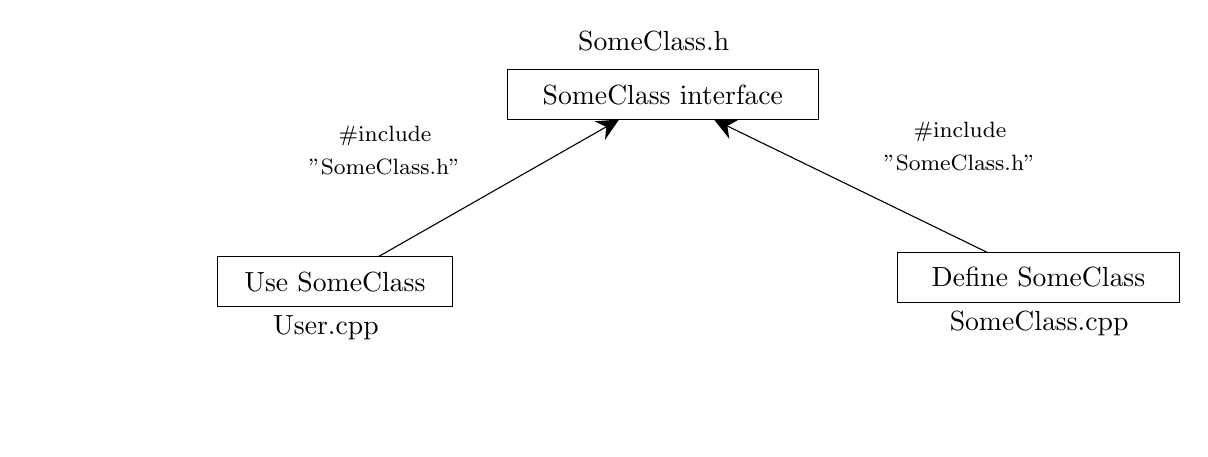
\begin{tikzpicture}[x=0.75pt,y=0.75pt,yscale=-1,xscale=1]
\centering
\path (0,235); %set diagram left start at 0, and has height of 235

% Text Node
\draw    (91.5,152) -- (204.5,152) -- (204.5,176) -- (91.5,176) -- cycle  ;
\draw (148,164) node    {Use\ \lstinline{SomeClass}};
% Text Node
\draw    (231,62) -- (381,62) -- (381,86) -- (231,86) -- cycle  ;
\draw (306,74) node    {\lstinline{SomeClass}\ interface};
% Text Node
\draw    (419,150) -- (555,150) -- (555,174) -- (419,174) -- cycle  ;
\draw (487,162) node    {Define\ \lstinline{SomeClass}};
% Text Node
\draw (117,179) node [anchor=north west][inner sep=0.75pt]   [align=left] {\lstinline{User.cpp}};
% Text Node
\draw (443,177) node [anchor=north west][inner sep=0.75pt]   [align=left] {\lstinline{SomeClass.cpp}};
% Text Node
\draw (264,42) node [anchor=north west][inner sep=0.75pt]   [align=left] {\lstinline{SomeClass.h}};
% Text Node
\draw (131,88) node [anchor=north west][inner sep=0.75pt]   [align=left] {\begin{minipage}[lt]{59.84pt}\setlength\topsep{0pt}
\begin{center}
{\footnotesize \lstinline{#include}\\{\footnotesize "SomeClass.h"}}
\end{center}

\end{minipage}};
% Text Node
\draw (408,86) node [anchor=north west][inner sep=0.75pt]   [align=left] {\begin{minipage}[lt]{59.84pt}\setlength\topsep{0pt}
\begin{center}
{\footnotesize \lstinline{#include}\\{\footnotesize "SomeClass.h"}}
\end{center}

\end{minipage}};
% Connection
\draw    (169.07,152) -- (282.33,87.48) ;
\draw [shift={(284.93,86)}, rotate = 510.33] [fill={rgb, 255:red, 0; green, 0; blue, 0 }  ][line width=0.08]  [draw opacity=0] (10.72,-5.15) -- (0,0) -- (10.72,5.15) -- (7.12,0) -- cycle    ;
% Connection
\draw    (462.32,150) -- (333.38,87.31) ;
\draw [shift={(330.68,86)}, rotate = 385.93] [fill={rgb, 255:red, 0; green, 0; blue, 0 }  ][line width=0.08]  [draw opacity=0] (10.72,-5.15) -- (0,0) -- (10.72,5.15) -- (7.12,0) -- cycle    ;

\end{tikzpicture}

The  code  in \lstinline{User.cpp} and \lstinline{SomeClass.cpp} shares the \lstinline{SomeClass} interface information presented in \lstinline{SomeClass.h}, but the two files are otherwise independent and can be separately compiled. 

\subsubsection{\lstinline{module} (C++20)} \label{modules}

\lstinline{#include}s are very old, error-prone,  rather expensive, and order dependent. In \lstinline{SomeClass.cpp}:

\begin{lstlisting}
module; // This compilation will define a module

// Here we put (include/define) stuff that SomeClass needs

export module SomeClass; // Defining the module called "SomeClass"

export class SomeClass { // Export this class
    public:
        SomeClass(int num);
        getNumber();
    private:
        int number;
};

SomeClass::SomeClass(int num): number = num { } // Because we export SomeClass, all its member functions (i.e. this constructor) are automatically exported

int SomeClass::getNumber() { return number; } // Exported as well

export double nonMemberFunction(const SomeClass& c) { return c.getNumber(); } // Non-member are not automatically exported, so we do this explicitly
\end{lstlisting}

We can then \lstinline{import SomeClass;} to use it on other files. \lstinline{import}s and \lstinline{#include}s can be freely used together.

The differences between headers and modules are not just syntactic:
\begin{itemize}[leftmargin=15pt,noitemsep,nolistsep]
\item A module is compiled once only (rather than in each translation unit in which it is used).
\item Two modules can be \lstinline{import}ed in either order without changing their meaning
\item If you \lstinline{import} something into a module, users of your module do not implicitly gain access to (and are not bothered by) what you imported;  \lstinline{import} is not transitive.
\end{itemize}

\subsubsection{\lstinline{namespace}} \label{namespace}
Another mechanism/scope for grouping declarations and making sure their names don't clash with others.

\begin{lstlisting}
namespace SomeNamespace {
    int main();
}

int SomeNamespace::main() {
    // Implementation
}

int main() { // Doesn't clash with 
    return SomeNamespace::main();
}
\end{lstlisting}

Standard-library names are in namespace \lstinline{std}. Names not local to a defined namespace, class, or function are in the global namespace. \lstinline{using std::swap} makes \lstinline{std::swap} usable as if it was declared in the scope in which it appears, i.e. no need for \lstinline{std::}. \lstinline{using namespace std;} makes the entire namespace available.

\subsection{Exception handling}
Compilers are optimized to make returning a value much cheaper than throwing the same value as an exception, but do not believe the myth that exception handling is slow; it is often faster than correct handling of complex or rare error conditions, and of repeated tests of error codes.

\subsubsection{\lstinline{throw}}
\lstinline|throw someException{"Error message"};| transfers control to a handler for exceptions of type \lstinline{someException} in the function that directly or indirectly called the current function.\\

\subsubsection{Standard library exceptions}

\begin{itemize}
    \item \lstinline{std::out_of_range}
    \item \lstinline{std::length_error}; when a non-positive number of elements is used to specify a sequence's length
    \item \lstinline{std::bad_alloc}; when operator \lstinline{new} can't find memory to allocate (memory exhaustion)
\end{itemize}

\subsubsection{\lstinline{try}-\lstinline{catch}}

\begin{lstlisting}
try { // Exceptions here are handled by the handler defined below
    // Code that may throw
}
catch (someException& exception) {
    std::cerr << exception.what() << '\n';
}
\end{lstlisting}

\lstinline{std::exception::what()} retrieves the error message.

\subsubsection{Re\lstinline{throw}}

\begin{lstlisting}
try {
    // Code that may throw
}
catch (someException& exception) {
    throw; // If this function can't complete its task, we can rethrow someException
}
\end{lstlisting}

\subsubsection{\lstinline{noexcept}}
A function that should never throw an exception can be declared \lstinline{noexcept}, e.g. \lstinline{void function() noexcept;}\\
If it still \lstinline{throw}s, \lstinline{std::terminate()} is called.

\subsubsection{Invariant}
A statement of what is assumed to be true for a class is called a class invariant, or simply an invariant. It is the job of a constructor to establish the invariant for its class (so that the member functions can rely on it) and for the member functions to make sure that the invariant holds when they exit.

\subsubsection{\lstinline{assert}}
\lstinline{assert(p != nullptr);} asserts that a condition (valid \lstinline{p}) must hold in at runtime. The program terminates when this fails in debug mode; in release mode \lstinline{assert}s aren't checked.

\subsubsection{\lstinline{static_assert}} \label{static_assert}
Like \lstinline{assert} but for compile time. Can be used for anything that can be expressed as a \hyperref[constexpr]{constant expression}, e.g.

\begin{lstlisting}
constexpr int minIntSize = 4;
static_assert(minIntSize <= sizeof(int), "Integers are too small."); // Writes "Integers are too small." as a compiler error message if an int on this system does not have at least 4 bytes
\end{lstlisting}

If you don't supply a message, the compiler will write a default message (typically the source location of the \lstinline{static_assert} plus a character representation of the asserted predicate) if the assertion fails. The most important uses of \lstinline{static_assert} come when we make assertions  about types used as parameters in generic programming.

\subsubsection{Resource  Acquisition  Is  Initialization (RAII)}
The technique of acquiring \hyperref[resource]{resources} in a constructor and releasing them in a destructor, thus making resource release guaranteed and implicit and avoiding allocations in general code and keep them buried inside the implementation of well-behaved abstractions. Let each resource have an owner in some scope and by default be released at the end of its owners scope.

In the C++ standard library, RAII is pervasive: for example, memory (\lstinline{std::string}, \lstinline{std::vector}, \lstinline{std::map}, \lstinline{std::unordered_map}, etc.), files (\lstinline{std::ifstream}, \lstinline{std::ofstream}, etc.), threads (\lstinline{std::thread}), locks (\lstinline{std::lock_guard}, \lstinline{std::unique_lock}, etc.), and general objects (through \lstinline{std::unique_ptr} and \lstinline{std::shared_ptr}).

\section{Types}

Types built out of other types using C++'s abstraction mechanisms.

\subsection{User-defined Types}

\subsubsection{Special member functions}

If a class \lstinline{X} has a destructor that performs a nontrivial task, such as free-store deallocation or lock release, the class is likely to need the full complement of special member functions:

\begin{lstlisting}
class X {
    public:
    X(int, SomeOtherType); // Constructor
    X(); // Default constructor
    X(const X&); // Copy constructor
    X(X&&); // Move constructor
    X& operator=(const X&); // Copy assignment: clean up target and copy
    X& operator=(X&&); // Move assignment: clean up target and move 
    ~X() // Destructor: clean up
    //...};
\end{lstlisting}

\subsubsection{\lstinline{=default} special member functions}

Except for the "ordinary constructor", the special member functions will be generated by the compiler as needed. If you want to be explicit about generating default implementations, you can by using 
\begin{lstlisting}
X(const X&) = default; // Enforce a default copy constructor
\end{lstlisting}

If you are explicit about some defaults, other default definitions will not be generated. Explicit copy and move operations are usually a good idea when a class has a pointer member, because a pointer may point to something that the class needs to (not) \lstinline{delete}, in which case the default memberwise copy would be wrong. A reader of the code would like to know. A good rule of thumb (sometimes called the \textit{rule of zero}) is to either define all of the essential operations or none (using the default for all). 

\subsubsection{\lstinline{=delete} member functions} \label{isdelete}

Indicates that an operation is not to be generated. A base class in a class hierarchy is the classical example where we don’t want to allow a memberwise copy. A \lstinline{=delete} makes an attempted use of the \lstinline{delete}d function a compile-time error; \lstinline{=delete} can be used to suppress any function, not just essential member functions.

\subsubsection{\lstinline{public} member}

Accessible to all code that can access/use the class of which it's a member.

\subsubsection{\lstinline{protected} member}

Accessible only to descendents of the class of which it's a member.

\subsubsection{\lstinline{private} member}

Accessible only to the class of which it's a member itself.

\subsubsection{\lstinline{struct}} \label{struct}

By default, members are \lstinline{public} in a \lstinline{struct}. By convention, \hyperref[struct]{\lstinline{struct}}s serve more as a bundle of data.

\begin{lstlisting}
struct Struct {
    int number;
};

Struct s;
s.number = 42; // Access through name (or reference)
Struct* sp = &s;
sp->number = 43; // Access through pointer
\end{lstlisting}

\subsubsection{\lstinline{class}} \label{class}

The only difference with a \hyperref[struct]{\lstinline{struct}} is that, by default, members are \lstinline{private} in a \lstinline{class} and that \lstinline{class}es inherit \lstinline{private}ly, whereas members default to \lstinline{public} in a \hyperref[struct]{\lstinline{struct}}. \lstinline{class}es are really meant for the notions of encapsulation and consolidating data and operations (on that data).

\begin{lstlisting}
class SomeClass {
    public: // Constitutes the interface
        // SomeClass() { }; is implicitly generated
        SomeClass(int num) : number = num { } // Constructor
        int getNumber() { return number; }
    private: // Only accessible via the interface
        int number;
};
\end{lstlisting}

\subsubsection{\lstinline{this}}

The name \lstinline{this} is predefined in a member function and points to the object for which the member function is called.

\subsubsection{Constructor}
A member "function" with the same name as its class is called a constructor; a function used to construct objects of a class. A constructor that can be invoked without an argument is called a \textit{default constructor}. A default constructor is implicitly generated if none is specified, which default initializes its members. A constructor of a derived class calls the constructor of its base class (implicitly in case there is a default constructor), meaning derived classes are constructed "bottom-up" (base first). Constructors don't [normally?] \lstinline{return} anything, but you can \lstinline{return} without an expression.

\begin{lstlisting}
SomeClass sc; // Default initialization/construction
SomeClass sc = SomeClass(42); // Initialization
\end{lstlisting}

\subsubsection{\lstinline{static} members} \label{staticmembers}

Member declaration specifier that declares members (variables or functions) that are not bound to class instances. They exist even if no objects of the class have been defined; hence they are referred to by their encapsulating class name rather than a specific variable name of its type. \lstinline{static} functions have no \lstinline{this} pointer. Only \lstinline{inline static} members may be defined in the class definition:

\begin{lstlisting}
struct X
{
    static void f(); // Function declaration. Cannot be defined in-class
    static int n;    // Variable declaration. Cannot be defined in-class
    inline static int in = 123; // Inline static member CAN be defined inline
};

int X::n = 69; // Variable definition
\end{lstlisting}

Outside a class definition, it has a different meaning.

\subsubsection{Initializer list} \label{initializerlist}
Notationally shorter way of initializing a class's member variables. Not to be confused with \hyperref[stdinitializerlist]{\lstinline{std::initializer_list}}.

\begin{lstlisting}
class Point { 
private: 
    int x; 
    int y; 
public: 
    Point(int i = 0, int j = 0) : x(i), y(j) {
        // Without the initializer list, we would have to do:
        // x = i;
        // y = j;
    } 
}; 
\end{lstlisting}

\lstinline{const} data members, reference variables, member objects that do not have a default constructor, and base class members must be initialized using an initializer list.

\subsubsection{Destructor}
A mechanism to ensure that the memory allocated by the constructor is deallocated.

\begin{lstlisting}
class SomeClass {
    public:
        ~SomeClass() { delete[] numbers; }
    private:
        int size;
        int* numbers;
};
\end{lstlisting}

Destructors are called automatically when variables of its type go out of scope or run out of lifetime. Destructors implicitly call the destructors of all member variables and base classes (meaning a derived class is destroyed "top-down", i.e. derived first) after the class body has run. Member variables are destructed in the opposite order they were constructed in, which is the order in which they appear in the class declaration. Constructor-destructor pairs are important to RAII.

\subsubsection{Conversion}

A constructor taking a single argument defines a conversion from its argument type, which then allows for implicit conversions.

\subsubsection{\lstinline{explicit} conversion}

In case we want to avoid implicit conversions caused by a single-parameter constructor, we prepend it with \lstinline{explicit} like so:

\begin{lstlisting}
explicit SomeClass(int num);
\end{lstlisting}

\subsubsection{Default member variables values}

\begin{lstlisting}
class SomeClass {
    int number = 42;
};
\end{lstlisting}

The default value is used whenever a constructor doesn’t provide a value.

\subsubsection{Copy}

By default, objects can be copied. The default meaning of copy is memberwise copy.

\begin{lstlisting}
SomeClass a = SomeClass(); // Default constructor initialization
SomeClass b{a}; // Copy initialization/construction (memberwise copy)
SomeClass c = a; // Copy assignment (memberwise copy)
\end{lstlisting}

\subsubsection{Copy constructor}

Used to initialize a previously uninitialized object (hence the name copy "constructor") from some other object's data. The default meaning of copy is memberwise copy, i.e. copying each member. For some sophisticated concrete types like resource handles or containers, memberwise copy is not the right semantics for copy; for abstract types it almost never is. For containers, the default copy would simply copy only the handle, leaving the two objects to refer to the same elements. We need our own copy constructor:

\begin{lstlisting}
SomeContainer::SomeContainer(const SomeContainer& sc) : numbers = new int[sc.size], size = sc.size {
    for (int i = 0; i != size; ++i) // Copy elements
        numbers[i] = sc.numbers[i];
}
\end{lstlisting}

\subsubsection{Copy assignment}

Used to replace the data of a previously initialized object with some other object's data. A copy constructor almost always needs a corresponding copy assignment operator definition:

\begin{lstlisting}
SomeContainer& SomeContainer::operator=(const SomeContainer& sc) {
    int* p = new int[sc.size];
    for (int i=0; i != sc.size; ++i)
        p[i] = sc.numbers[i];
    delete[] numbers; // Delete old elements
    numbers = p;
    size = sc.size;
    return *this;
}
\end{lstlisting}

Default copy assignment does a simple memberwise copy, which for pointer and handles can cause memory leaks (hence they are often \hyperref[isdelete]{\lstinline{=delete}d} for such types).

\subsubsection{Move constructor} \label{moveconstructor}

\lstinline{return}ing large values is expensive if they need to be copied out of a function while there is no move constructor. Defining a move constructor allows data to be efficiently moved out of a function:

\begin{lstlisting}
SomeContainer::SomeContainer(SomeContainer&& sc) : numbers = sc.numbers, size = sc.size {
    sc.numbers = nullptr;
    sc.size = 0;
}
\end{lstlisting}

A move operation is applied when an \hyperref[rvaluereference]{rvalue reference} is used as an initializer or as the right-hand side of an assignment. This means that \lstinline{return}ing an object of a type with a move constructor gets moved out of the function instead of copied out of it. After a move, a moved-from object should be in a state that allows a destructor to be run.  Typically, we also allow assignment to a moved-from object.

\subsubsection{\lstinline{std::move()}}
Where the programmer knows that a value will not be used again, but the compiler can't be expected to be smart enough to figure that out, you can use \lstinline{std::move()} to get an \hyperref[rvaluereference]{rvalue reference} to its argument from which we may move; it doesn't actually move anything, but essentially casts an lvalue to an \hyperref[rvaluereference]{rvalue reference} (it really should have been called \lstinline{rvalue_cast} or something).

\begin{lstlisting}
Vector someFunction() {
    // Initialize ints x, y, z
    z = x; // Copy (because x might be used later in someFunction())
    y = std::move(x); // Move (assignment), so x should not be used anymore
    // ... better not use x here ...
    return z; // Move
}
\end{lstlisting}

The state of a moved-from object is in general unspecified, but all standard-library types leave a moved-from object in a state where it can be destroyed and assigned to, e.g. \lstinline{std::vector}s and \lstinline{std::string}s are empty. For many types, the default value is fine as replacement.

Like other casts, it’s error-prone and best avoided. Use only if you can demonstrate significant and necessary performance improvement. It exists to serve a few essential cases, e.g. a simple three-step swap operation, where we don't want to copy three times.

\subsubsection{Move assignment} \label{moveassignment}

A move constructor [almost?] always needs a corresponding move assignment operator definition:

\begin{lstlisting}
SomeContainer& SomeContainer::operator=(const SomeContainer& sc) {
    int* p = new int[sc.size];
    for (int i=0; i != sc.size; ++i)
        p[i] = sc.numbers[i];
    delete[] numbers; // Delete old elements
    numbers = p;
    size = sc.size;
    return *this;
}
\end{lstlisting}

\subsubsection{\lstinline{std::initializer_list}} \label{stdinitializerlist}

Not to be confused with \hyperref[initializerlist]{a constructor's initializer list}.

When we use a \lstinline|{}|-list, such as \lstinline|{1,2,3,4}|, the compiler will create an object of type \lstinline{initializer_list}, which can be used to construct containers with.

\begin{lstlisting}
class SomeContainer {
    public:
        SomeContainer(std::initializer_list<double> list) : numbers = new int[list.size()], sz = static_cast<int>(lst.size()); { copy(list.begin(), list.end(), numbers) } // Initialize with a list of int
    private:
        int size;
        int* numbers; // numbers points to an array of ints of size size
}

SomeContainer sc = {1,2,3};
\end{lstlisting}

Unfortunately, the standard-library uses \lstinline{unsigned} integers for sizes and subscripts, so you need to use the ugly \hyperref[staticcast]{\lstinline{static_cast}} to explicitly convert the size of the \lstinline{std::initializer_list} to an \lstinline{int}, even though the chance that the number of elements in a handwritten list is larger than the largest integer is rather low. 

\subsubsection{\lstinline{union}}
A \lstinline{struct} in which all members are allocated at the same address, so that the \lstinline{union} occupies only as much space as its largest member.

\begin{lstlisting}
union Value {
    Node* p;
    int i;
};
\end{lstlisting}

Naturally, a \lstinline{union} can hold a value for only one member at a time, so the programmer must keep track for which variable the value is held (or the different variables must share the same bit representation).

\subsubsection{\lstinline{std::variant<>}}
A type-safe standard library wrapper around \lstinline{union} which is less error-prone.

\begin{lstlisting}
std::variant<int, float> v = 42; // v holds an int
bool isInt = holds_alternative<int>(v); // true
int w = std::get<int>(v);
int w = std::get<0>(v); // same effect as the previous line
int w = std::get<float>(v); // throws std::bad_variant_access
\end{lstlisting}

\subsubsection{\lstinline{std::visit<>()}}

Calls a \hyperref[functors]{functor} (function object) -- called the \emph{visitor} -- on the value currently contained in a \lstinline{variant}. The \hyperref[functors]{functor} is a \lstinline{class} or \lstinline{struct} whose \lstinline{operator()} is overloaded for each type of the \lstinline{variant}, so that it can actually be called on all possible types.

\subsubsection{\lstinline{enum}} \label{enum}
A mnemonic representation of small sets of integer values, used to make code more readable and less error-prone than if we had to use the \lstinline{int}s directly. Enumerators from a (plain) \lstinline{enum} are entered into the same scope as the name of their \lstinline{enum} and implicitly converts to their integer value, hence they're also referred to as unscoped enums.

\begin{lstlisting}
enum Color { red, blue };
enum Traffic_light { green, yellow }; // We cannot redefine red or blue; they're in the same scope

bool sameInt = Color::red == Traffic_light::green; // true; they're both 0
Color c = 1; // Same as Color c = Color::red /  Color c = red;
\end{lstlisting}

\subsubsection{\lstinline{enum class}}
The difference with \hyperref[enum]{\lstinline{enum}} is that the enumerators are in the scope of their \lstinline{enum class} instead of outside of it, so they can be used repeatedly in different \lstinline{enum class}es without confusion, but enumerators from different \lstinline{enum class}es -- as well as enumerators and \lstinline{int}s -- can't be freely mixed anymore. Also called scoped enums.

\begin{lstlisting}
enum class Color { red, blue, green };
enum class Traffic_light { green, yellow, red }; // We can now use the same enumerator in different enums
\end{lstlisting}

Since an enumeration is a user-defined type, we can define operators for it:

\begin{lstlisting}
Traffic_light& operator++(Traffic_light& t)//prefix increment: ++ {
    switch (t) {
        case Traffic_light::green: return t=Traffic_light::yellow;
        case Traffic_light::yellow: return t=Traffic_light::red;
        case Traffic_light::red: return t=Traffic_light::green;
    }
}
\end{lstlisting}

Using \lstinline{enum struct} is exactly the same.

\subsubsection{\lstinline{std::underlying_type<>}}

A templated \hyperref[struct]{\lstinline{struct}} which -- if supplied with a complete enumeration type (either \lstinline{enum} or \lstinline{enum class}) -- provides a \hyperref[typedef]{\lstinline{typedef}} member called \lstinline{type} that gives the underlying type of the enumeration type (which by default is \lstinline{int} for scoped enumerations and some implementation specific integral type for unscoped enumerations).\\
If you want another underlying type for an enumeration type, you have to explicitly declare this:

\begin{lstlisting}
enum class e: unsigned {}; // Uses unsigned ints as underlying type
\end{lstlisting}

\subsubsection{\lstinline{decltype()}}

Returns the type of an expression. If given the name of a variable (an "id-expression"), it returns the type of the variable, if given an lvalue of type \lstinline{T}, it returns \lstinline{T&}, and if given an rvalue of type \lstinline{T}, it returns \lstinline{T}.

\begin{lstlisting}
int n = 10;
decltype(n) a = 20; // a is an int
decltype((n)) b = a; // b is an int&, because (n) is an lvalue
\end{lstlisting}

\subsection{Inheritance}

\subsubsection{\lstinline{virtual} function} \label{virtual}

\begin{lstlisting}
class SomeClass {
    public:
        virtual int& getNumber() const { return number; }; // Virtual function
    private:
        int number;
}
\end{lstlisting}

\lstinline{virtual} indicates that a class deriving the current class may redefine this function, in which case this more specific implementation is called on objects of the derived class, even if those are declared as the base class. The base class must provide a definition of a \lstinline{virtual} function, which serves as the default function for all derived classes that don't reimplement it.

\subsubsection{Pure \lstinline{virtual} function} \label{purevirtual}

Putting \lstinline{= 0} behind a \lstinline{virtual} function declaration makes it purely virtual. Having a pure virtual function makes a class abstract, meaning it can't be instantiated. A concrete deriving/inheriting class \emph{must} (re)implement any pure virtual functions; if they don't, they become abstract as well.

\begin{lstlisting}
class AbstractBase {
    public:
        virtual void function() const = 0; // Pure virtual function
    private:
        int number;
}

AbstractBase ab; // Error: there can be no objects of an abstract class
AbstractBase c = new Child(10); // OK: AbstractBase is a base class/interface for Child
\end{lstlisting}

A base class can still give a definition, however. An example of a use case for this is when there is a reasonable default behaviour, but the designer only wants this behaviour to be called explicitly, i.e. the base class's implementation must be explicitly called from the derived implementation:

\begin{lstlisting}
class Child : public AbstractBase { // AbstractBase's declaration of function() would have to be public or protected to avoid a compile time problem

    virtual void function() {
        AbstractBase::function(); // Class Child doesn't have anything special to do for function() so we'll call AbstractBase's
    }

};
\end{lstlisting}

\subsubsection{Concrete types}
Types of which the representation is part of the definition, i.e. they have no \hyperref[purevirtual]{pure \lstinline{virtual} functions}. Can be instantiated.

\subsubsection{Abstract types}
A type that completely insulates a user from implementation details. The interface is decoupled from the representation, and genuine local variables are given up. Since we don't know anything about the representation of an abstract type (not even its size), we must allocate objects on the free store and access them through references or pointers.

More concretely, abstract types are types with at least one \hyperref[purevirtual]{purely \lstinline{virtual}} function, and such classes cannot be instantiation; they can only be inherited from by other, potentially concrete classes.

A virtual destructor is essential for an abstract class, because an object of a derived class is usually manipulated through the interface provided by its abstract base class (i.e. a pointer to the base type), and someone destroying an abstract container class through a pointer has no idea what resources are owned by this derived implementation. Then, the virtual function call mechanism ensures that the proper destructor is called. That destructor then implicitly invokes the destructors of its members and bases, so that objects are destroyed "top-down".

A class that provides the interface to a variety of other classes is often called a \textit{polymorphic type}. Polymorphic functions (having an (abstract) base class as parameter type) needn't be recompiled if the implementation of a derived class of the parameter type changes or a brand-new class is derived. The flip side of this flexibility is that objects must be manipulated through pointers or references.

\subsubsection{Inheritance}

Classes in class hierarchies are different from concrete, singular classes: we tend to allocate them on the free store using \lstinline{new}, and we access them through pointers or references. Two benefits are \textit{interface inhertiance} (an object of a derived class can be used wherever an object of a base class is required; the base class acts as an interface for the derived class) and \textit{implementation inheritance}.

\begin{lstlisting}
class DerivedClass : public BaseClass { // BaseClass can be either abstract or concrete
    public:
        virtual int& getNumber() override { return number; }; // Override a function that base class defines as well
    private:
        int number;
}
\end{lstlisting}

\subsubsection{Kinds of inheritance}

The \lstinline{public}/\lstinline{protected}/\lstinline{private} keyword after the \lstinline{:} decides what code is "aware of" the inheritance:

\begin{lstlisting}
class Base
{
    public:
        int x;
    protected:
        int y;
    private:
        int z;
};

class ChildA : public Base
{
    // x is public
    // y is protected
    // z is not accessible from ChildA
};

class ChildB : protected Base
{
    // x is protected
    // y is protected
    // z is not accessible from ChildB
};

class ChildC : private Base    // 'private' is default for classes
{
    // x is private
    // y is private
    // z is not accessible from ChildC
};
\end{lstlisting}

\lstinline{ClassA}, \lstinline{ClassB} and \lstinline{ClassC} all contain the variables \lstinline{x}, \lstinline{y} and \lstinline{z}. It is just question of access. If a concrete class is derived from another concrete class, its constructor [always?] calls the constructor of its parent class, either implicitly through a default constructor or in the \hyperref[initializerlist]{initializer list} in case we need to supply arguments.

\subsubsection{\lstinline{override}}

Optional keyword used to make explicit to readers and the compilers (so that it can catch spelling errors or type differences) that the current function definition overrides the base class's definition. It's not actually needed, though.

\subsubsection{Virtual function table}

A mechanism for \textit{dynamic dispatch}, i.e. resolving which function implementation to use when a function is called on an object declared as a base type. The usual implementation technique is for the compiler to convert the name of a virtual function into an index into a table of pointers to functions, called the virtual function table or simply the \lstinline{vtbl}. Each class with virtual functions has its own \lstinline{vtbl} identifying its virtual functions. The implementation of the caller needs only to know the location of the pointer to the \lstinline{vtbl} in a base class and the index used for each virtual function. This virtual call mechanism can be made almost as efficient as the "normal function call" mechanism (within 25\%). Its space overhead is one pointer in each object of a class with virtual functions plus one \lstinline{vtbl} for each such class.

\subsubsection{Class hierarchy}

A set of classes ordered in a lattice created by derivation. We use class hierarchies to represent concepts that have hierarchical relationships.

\subsubsection{\lstinline{dynamic_cast}}

Attempts to cast the runtime type of a variable. We can use this to determine whether the pointer to the base type is at runtime actually some derived type, e.g. in order to use a member function that is only provided by a particular derived class:

\begin{lstlisting}
Base* pb;
// pb changes during runtime
if (Derived* pd = dynamic_cast<Derived*>(pb)) {
    // pd points to a Derived; use it
}
\end{lstlisting}

If at runtime the object pointed to by the argument of \lstinline{dynamic_cast} (\lstinline{pb}, a \lstinline{Base*}) is not of the expected type (\lstinline{Derived*}) or a class derived from the expected type, \lstinline{dynamic_cast} returns \lstinline{nullptr}.

When a different type is unacceptable, we can simply \lstinline{dynamic_cast} to a reference type. If the object is not of the expected type, \lstinline{dynamic_cast} throws a \lstinline{std::bad_cast} exception:

\begin{lstlisting}
Derived& r {dynamic_cast<Derived&>(*pb)};   // Catch std::bad_cast somewhere
\end{lstlisting}

\subsection{Container}

A \lstinline{struct} or \lstinline{class} that serves as a \textit{resource handle} (a class responsible for an object accessed through a pointer) to a collection of elements elsewhere, e.g. a \lstinline{class} that manages an array in dynamic memory using \lstinline{new} and \lstinline{delete}.

\subsubsection{std::vector<>} \label{std_vector}

The most common standard library container type. Its elements are stored contiguously in memory on the heap/free store. A vector holds pointers to the first element, one-past-the-last element, one-past-the-last allocated space, and an allocator responsible for acquiring and releasing memory through \hyperref[new]{\lstinline{new}} and \hyperref[delete]{\lstinline{delete}}. \lstinline{size()} is a member function giving the number of elements. Subscripting with \lstinline{[]} is supported but doesn't range-check due to overhead; \lstinline{at()} does the same thing but with range-checking, i.e. throwing an exception of type \lstinline{out_of_range}. \lstinline{push_back()} adds an element to the end of the vector. \lstinline{emplace_back()} takes arguments for an element’s constructor and constructs it in a newly allocated space in the container, avoiding copying it.

\begin{lstlisting}
// Allocation initialization
std::vector<bool> bools(3); // Contains 3 default-constructed bools
std::vector<bool> nobools; // Contains 0 bools

// List initialization
std::vector<int> ints = {1, 2, 3, 4, 5};

// Equivalued initialization
vector<bool> vect(10, true); // Contains 10 booleans that are all true

// Declaration and loop push_back
std::vector<int> ints;
for (int i = 0; i < 10; ++i) {
    ints.push_back(i);
}

// Range-for loops are supported
void print_book(const vector<int>& ints) {
for (const auto& x : book)
    // ...
}
\end{lstlisting}

Copying or assigning a \lstinline{std::vector} involves copying its elements.

\lstinline{std::vector<bool>} is a special optimization, which stores each boolean in one bit instead of the usual 8. This saves a lot of memory, but makes a lot of the usual \lstinline{std::vector} operation, like \lstinline{operator[]} and \lstinline{data()} unavailable.

Do not store objects of polymorphic type in a container directly, because specializations may increase the size; instead, use pointers.

\lstinline{std::vector}s are highly efficient, and you should almost always use these over regular arrays. When doubting its performance, measure. Subscripting and traversal are cheap and easy, but insertion and deletion may involve moving all elements to another place in memory. Returning a vector is efficient because vector provides move semantics.

\subsubsection{\lstinline{std::list<>}} \label{std_list}

A doubly-linked list. Meant for sequences where we want to insert and delete elements without moving other elements. Useful when requiring many \lstinline{insert(T* elem, T elemNew)} and \lstinline{erase(T* elem)} operations.

\subsubsection{\lstinline{std::forward_list<>}} \label{std_forward_list}

A singly-linked list. Allows only forward iteration, but saves space by not storing a pointer to the previous element. Doesn't even keep track of its number of elements, contrary to \lstinline{std::list}.

\subsubsection{\lstinline{std::map<>}} \label{std_map}

A balanced binary search tree that associates, or maps, keys to values and stores those as pairs. Subscripting a map with a key type return the associated value if found, or creates a new pair with a default constructed value. You can also use \lstinline{find()} and \lstinline{insert()}. Lookup is $O(\log n)$.

\subsubsection{\lstinline{std::unordered_map<>}} \label{std_unordered_map}

Uses a hash table and doesn't require an ordering function, hence the name. It does require a hash function as second template variable. C++ provides hasing function for built-in types and \lstinline{std::string}s as function objects. For user-defined types, creating a new hash function by combining existing hash functions using exclusive-or (\lstinline{^}) is simple and often very effective. You can do this by specializing the standard library \lstinline{hash}:

\begin{lstlisting}
template<> struct hash<Record> {
    using argument_type = Record;
    using result_type = std::size_t;
    
    size_t operator()(const Record& r) const {
        return hash<string>()(r.name) ^ hash<int>()(r.product_code);
    }
}
\end{lstlisting}

An \lstinline{unordered_map} is much faster than a \lstinline{map} for large containers when using a good hash function, but worst-case performance is far worse when using a bad one.

\subsubsection{\lstinline{std::multimap<>}} \label{std_multimap}

A \hyperref[std_map]{\lstinline{std::map}} in which a value can occur multiple times.

\subsubsection{\lstinline{std::set<>}} \label{std_set}

A \hyperref[std_map]{\lstinline{std::map}} with just keys and no values, i.e. a sorted collection of unique elements.

\subsubsection{\lstinline{std::multiset<>}} \label{std_multiset}

A \hyperref[std_set]{\lstinline{std::set}} in which a value can occur multiple times.

\subsubsection{\lstinline{std::unordered_set<>}} \label{std_unordered_set}

A \hyperref[std_set]{\lstinline{std::set}} with using hashed lookup.

\subsubsection{\lstinline{std::deque<>}} \label{std_deque}

A double-ended queue.

\subsubsection{\lstinline{size()}}

Conventional member function of container classes for getting the number of elements it holds.

\subsubsection{\lstinline{begin()}} \label{begin}

Conventional member function of container classes for getting an iterator pointing to the first element. Implementation may looks sorta like:

\begin{lstlisting}
template<typename T>
T* begin(SomeContainer<T>& x) {
    return x.size() ? &x[0] : nullptr; // Pointer to first element or nullptr
}
\end{lstlisting}

\subsubsection{\lstinline{end()}}

Conventional member function of container classes for getting an iterator pointing to the one-beyond-the-last element. Implementation may looks sorta like:

\begin{lstlisting}
template<typename T>
T* end(SomeContainer<T>& x) {
    return x.size() ? &x[0] + x.size() : nullptr;
}
\end{lstlisting}

\subsubsection{Iterator}

Each container type has an associated iterator of type \lstinline{C::iterator}. Even though their implementation may differ greatly (because the containers themselves differ), they all share the same semantics and operators, so that they may essentially be used as a pointer to a container's elements. They are used to traverse a sequence/container or to pass (sub)sequences to other functions.  Should support \lstinline{++} to move to the next element and \lstinline{*} to access the value of the element pointed to. Iterators are \hyperref[concepts]{concepts}.

\subsubsection{\lstinline{std::hash<K>} and \lstinline{std::unordered_map<K,V>} types}

The standard-library \lstinline{std::unordered_map<K,V>} is a hash table with \lstinline{K} as the key type and \lstinline{V} as the value type. To use a type \lstinline{K} as a key, we must define \lstinline{hash<K>}. The standard library does that for us for common types, such as \lstinline{std::string}.

\subsection{Templates}

Compile-time mechanism (i.e. no run-time overhead) for parametrizing a class:

\begin{lstlisting}
template<typename T> // Makes T a parameter of the declaration it prefixes
class SomeContainer {
    private:
        T* elem; // Elem points to an array of sz elements of type T
    public:
        // Constructor, destructor, etc. etc.
        T& operator[](int i);
}
\end{lstlisting}

or a member function:

\begin{lstlisting}
template<typename T> // Basically means "for all types T"
SomeContainer<T>::SomeContainer(int size) {
    if (size < 0)
        throw Negative_size{};
    elem = new T[size];
}
\end{lstlisting}

We can then \textit{instantiate}/\textit{specialize} these:

\begin{lstlisting}
SomeContainer<std::string> sc(17); // SomeContainer of 17 strings
\end{lstlisting}

\subsubsection{\lstinline{typename}}

Keyword used to introduce a type parameter (in \lstinline{template<typename T>}).

\subsubsection{\lstinline{class}}

Equivalent to \lstinline{typename} (e.g. \lstinline{template<class T>}). Found more in older code.

\subsubsection{Value template arguments}

Template value arguments must be constant expressions.

\begin{lstlisting}
template<typename T, int N>
\end{lstlisting}

\subsubsection{Read-only access to template arguments} \label{readonlyaccesstotemplatearguments}

It is very common for a parameterized type to provide an \hyperref[alias]{alias} for types related to their template arguments:

\begin{lstlisting}
template<typename T, int N>
struct Buffer {
    using value_type = T; // Alias to get the type T
    constexpr int size() { return N; } // constexpr function to get the value N
    T[N];
}
\end{lstlisting}

Every standard-library container provides \lstinline{value_type} as the name of its value type. The aliasing mechanism can be used to define a new template by binding some or all template arguments:

\begin{lstlisting}
template<typename Key, typename Value>
class Map {
    // ...
};

template<typename Value>
using StringMap = Map<std::string, Value>;

StringMap<int> m; // m is a Map<std::string, int>
\end{lstlisting}

\subsubsection{Default template arguments} \label{default_template_arguments}

\begin{lstlisting}
template<typename T1, typename T2 = T1> // If we don't supply a second argument, the types will be equal
\end{lstlisting}

\subsubsection{Template argument deduction (C++17)}

Instead of

\begin{lstlisting}
pair<int,double> p = make_pair(1,5.2); // p is a pair<int,double>
\end{lstlisting}

we can do

\begin{lstlisting}
pair p = {1,5.2}; // p is a pair<int,double>
\end{lstlisting}

So we don't need to annoyingly specify the template parameters.

\subsubsection{Deduction guides}

In case that the compiler cannot deduce template arguments -- such as when a custom \lstinline{Vector} type is range-initialized with a beginning and end iterator -- we can add a \emph{deduction guide} after the constructor:

\begin{lstlisting}
template<typename Iter>
Vector(Iter, Iter) -> Vector<typename Iter::value_type>
\end{lstlisting}

So now, when a \lstinline{Vector} is initialized with two iterators from any container datatype (including \lstinline{Vector} itself), it will automatically deduce to the iterator's value type.

\subsubsection{Variable templates}

\begin{lstlisting}
template <class T>
constexpr T viscosity = 0.4;

template <class T>
constexpr space_vector<T> external_acceleration = { T{}, T{-9.8}, T{} };

auto vis = 2 * viscosity<double>;
auto acc = external_acceleration<float>;
\end{lstlisting}

\subsubsection{Variadic templates} \label{variadictemplates}

Allows a template to take an arbitrary number of arguments of arbitrary type. Concretely, a variadic template has at least one \emph{parameter pack}, indicated by \lstinline{...}:

\begin{lstlisting}
template<typename... Ints>
void function(Ints... ints) {
   int args[] { ints... }; // Unpack ints here
}
\end{lstlisting}

For example:

\begin{lstlisting}
template<typename Head, typename... Tail> // Tail is a sequence of types
void print(Head head, Tail... tail) {// tail is a sequence of values of the types in Tail
    cout << head << ' ';
    print(tail...); // Don't forget to catch for an empty parameter list
}
\end{lstlisting}

Similar to \hyperref[variadicarguments]{variadic arguments}.

\subsubsection{Fold expressions (C++17)}

Shorthand notation using \lstinline{...} that compounds the arguments in a \hyperref[variadictemplates]{variadic template}. Examples:

\begin{lstlisting}
template<Number... T>
int sum(T... v) {
    return (0 + ... + v); // Left fold: (((((0+v[0])+v[1])+v[2])+v[3])+v[4]). OR:
    return (v + ... + 69); // Right fold: (v[0]+(v[1]+(v[2]+(v[3]+(v[4]+69)))))
}

template<typename ...T>
void print(T&&... args) {
    (std::cout << ... << args); // Print all arguments
}

template<typename T, typename... Ts>
vector<T> to_vector(Ts&&... ts)
{
    vector<T> res;
    (res.push_back(ts) ...);
    return res;
}
\end{lstlisting}

\subsubsection{\lstinline{std::forward<>()}ing arguments}

\begin{lstlisting}
template<typename T>
void intermediary(T&& arg) 
{
    destination(std::forward<T>(arg));
}
\end{lstlisting}

\lstinline{std::forward<T>(arg)} forwards \lstinline{arg} (which is always an lvalue) as either an lvalue or as rvalue, depending on \lstinline{T}. It moves/forwards the arguments unchanged, and is essentially a more sophisticated \href{}{\lstinline{std::move()}} by correctly handling subtleties to do with lvalue and rvalue. Use \lstinline{std::forward()} exclusively for forwarding and don't \lstinline{std::forward()} something twice; once you have forwarded an object, it's not yours to use anymore.

\subsubsection{Template compilation}

Argument checking for unconstrained template arguments is postponed until code is generated for the template and a set of template arguments, i.e. at (template) instantiation time. This late checking has two disadvantages:

\begin{itemize}
    \item Type errors can be found uncomfortably late and with difficult error messages, because the compiler found the problem only after combining information from several places in the program.
    \item We have to resort to \emph{duck typing}, i.e. we check with respect to values rather than object types.
\end{itemize}

To use an unconstrained template, its definition (not just its declaration) must be in scope at its point of use. In practice, this means that template definitions are typically found in header files, rather than \lstinline{.cpp} files. This changes when we start to use \hyperref[modules]{modules}, in which case the source code is organized in the same way for ordinary functions and template functions.

\subsection{Concepts (C++20)} \label{concepts}

Constrained template arguments, or, requirements on template arguments, or, predicates that check whether template argument \lstinline{T} has all the properties that whatever it prefixes requires (else it throws a compile-time error). Concepts are abstractions representing the fundamental operations and data structures (i.e. concepts) that \emph{generic programming} aims to abstract away from and into generic algorithms applicable on a wide variety of data structures. The process of generalizing from concrete code while preserving performance is called \emph{lifting}, and often simply entails replacing concrete types with template arguments.\\
Concepts help with catching errors during compile-time. For example, when we need a sequence:

\begin{lstlisting}
template<Sequence T> // "For all T such that Sequence(T)"
\end{lstlisting}

which is equivalent to

\begin{lstlisting}
template<typename T>
requires Sequence<T> // Requires that T is a Sequence
\end{lstlisting}

Here, \lstinline{Sequence} is a predicate, or a \emph{concept}. Other predicates are \lstinline{Element}, which checks whether a type has all the properties that a vector requires of its elements.

\subsubsection{Standard library concepts}

A small selection:
\begin{itemize}
    \item \lstinline{Element}; a type with all properties that a vector requires of its elements.
    \item \lstinline{Regular}; is \lstinline{DefaultConstructible}, \lstinline{Copyable}, \lstinline{EqualityComparable}, and doesn't suffer from technical problems due to overly clever programming tricks.
    \item \lstinline{Semiregular}; only \lstinline{DefaultConstructible} and \lstinline{Copyable}.
    \item \lstinline{Copyable}; \lstinline{CopyConstructable}, \lstinline{Moveable} and \lstinline{Assignable}.
    \item \lstinline{StrictTotallyOrdered}; can be compared with \lstinline{<}, \lstinline{<=}, \lstinline{>} and \lstinline{>=}.
    \item \lstinline{Range}; a sequence of element, defined by either \lstinline{begin()} and \lstinline{end()}, or \lstinline{begin()} and a number $n$ of elements, or \lstinline{begin()} and a predicate that is \lstinline{true} for the end-of-sequence. Thanks to this concept, where a standard-library algorithm requires a sequence defined by a pair of iterators, C++20 will allow a \lstinline{Range} as a notationally simpler alternative (e.g. \lstinline{std::sort(v)} rather than \lstinline{sort(v.begin(),v.end())}). 
\end{itemize}

\subsubsection{\lstinline{requires}-clause}

The \lstinline{requires}-clause specifies a requirement on the template parameter. This \textit{constrained argument} specifies a \textit{constrained template}. The \lstinline{typename} introducer requires only that the argument is a type. 

A more complete example:

\begin{lstlisting}
template<Sequence Seq, Number Num> // We should define what Sequence and Number mean
requires Arithmetic<Value_type<Seq>, Num> // We need to be able to add the element type of Seq (Value_type<Seq>) to the type of the accumulator (Num)
Num sum(Seq s, Num v) {
    for (const auto& x : s) v+=x;
    return v;
}
\end{lstlisting}

This can be written more verbose:

\begin{lstlisting}
template<typename Seq, typename Num>
requires Sequence<Seq> && Number<Num> && requires Arithmetic<Value_type<Seq>, Num>
Num sum(Seq s, Num n);
\end{lstlisting}

or even less verbose:

\begin{lstlisting}
template<Sequence Seq, Arithmetic<Value_type<Seq>> Num>
Num sum(Seq s, Num n); // Num is a patially specified requirement
\end{lstlisting}

\subsubsection{\lstinline{requires}-expression}

Used within a \lstinline{requires}-clause, yielding \lstinline{true} if the statements in it are valid code and \lstinline{false} if they're not.

\begin{lstlisting}
template<Forward_iterator Iter, int n>
requires requires(Iter p, int i) { p[i]; p+i; } // Iter has subscripting and addition
void advance(Iter p, int n) // move p n elements forward
{
    p += n; // A random-access iterator has +=
}
\end{lstlisting}

However, if you see \lstinline{requires requires} in your code, it is probably too low level; \lstinline{requires}-expressions are the assembly code of generic programming. Prefer use of properly named concepts with well-specified semantics, and use \lstinline{requires}-expressions in the definition of those.

\subsubsection{Concept-based overloading}

We can overload function that have the same type (i.e. same arguments and return type) based only on their template concept. This means that we have different function bodies for different template concepts. The compiler will select the template with the strongest requirements met by the template arguments. Like regular overloading, this is also a compile-time mechanism.

\subsubsection{Defining \lstinline{concept}s}

Besides the concepts provided in the standard library and other libraries, we can define our own. For example, if we want to define a concept for types that are equality comparable:

\begin{lstlisting}
template<typename T1, typename T2 = T1> // Default template argument
concept Equality_comparable = requires (T1 a, T2 b) {
    { a == b } -> bool; // Compare a T1 to a T2 with ==
    { a != b } -> bool; // Compare a T1 to a T2 with !=
    { b == a } -> bool; // Compare a T2 to a T1 with ==
    { b != a } -> bool; // Compare a T2 to a T1 with !=
};
\end{lstlisting}

For each line in the  \lstinline{requires}-body, the expression inside the \lstinline|{ }| must be correct and must yield the type behind the \lstinline{->}. Using \hyperref[default_template_arguments]{default template arguments}, we only need to supply one type. If we only supported comparing the same type, the \lstinline{requires}-body would be only two lines.

We can test using \hyperref[static_assert]{\lstinline{static_assert}}:

\begin{lstlisting}
static_assert(Equality_comparable<int,string>); // Fails
\end{lstlisting}

A more complicated example:

\begin{lstlisting}
template<typename S>
concept Sequence = requires(S a) {
    typename Value_type<S>; // S must have a value type.
    typename Iterator_type<S>; // S must have an iterator type.
    { begin(a) } -> Iterator_type<S>; // begin(a) must return an iterator
    { end(a) } -> Iterator_type<S>; // end(a) must return an iterator
    requires Same_type<Value_type<S>,Value_type<Iterator_type<S>>>;
    requires Input_iterator<Iterator_type<S>>;
};
\end{lstlisting}

\section{Functions}

\subsection{Function templates}

\begin{lstlisting}
template<typename Sequence, typename Value>
Value sum(const Sequence& s, Value v) { // v is initial value of the accumulator
    for (auto x : s) v += x;
    return v;
}

std::list<double>& ld;
// ...
double sum = sum(ld,0.0); // Types of the template arguments are deduced from function arguments
\end{lstlisting}

Member functions can be function templates, but a \lstinline{virtual} members cannot. (The compiler would not know all instantiations of such a template in a program, so it could not generate a \lstinline{vtbl}).

\subsection{Function objects/functors} \label{functors}

Also called \textit{functors}. Objects that can be called like functions, implemented as a class with a function call operator \lstinline{operator()}:

\begin{lstlisting}
template<typename T>
class LessThan {
    const T val; // Value to compare against
    public:
        LessThan(const T\& v) : val{v} { } // Constructor
        bool operator()(const T\& x) const { return x < val; }  // Call operator
}

LessThan lti {42}; // lti(i) will compare i to 42. Template argument is deduced
LessThan<std::string> lts {"Naur"}; // "Naur" is a C-style string, so we need <std::string> to get the right <

bool b1 = lti(12); // True
bool b2 = lts("Zzz"s); // False
\end{lstlisting}

Function objects are widely used as arguments to algorithms to serve as predicates.

\subsection{Lambda expressions}

Defines an unnamed function at the place of its use with notation \lstinline|[]{ }|, e.g. \lstinline|[&](int a){ return a<x; }|. The \lstinline{[&]} is a capture list specifying that all local names (from outside the lambda) used in the lambda body (such as \lstinline{x}) will be accessed through references. If you want to reference only \lstinline{x}, you can specify this using \lstinline{[&x]}. For copying \lstinline{x}: \lstinline{[=x]}. Capturing nothing is \lstinline{[]}, capture all local names used by reference is \lstinline{[&]}, and capture all local names used by value is \lstinline{[=]}.

A \textit{generic lambda} is essentially a templated lambda; a lambda with an \lstinline{auto} parameter, meaning that any type is accepted as an initializer. (For reasons lost in standards committee politics, this use of \lstinline{auto} is not currently allowed for function arguments.)

\subsection{Variadic arguments} \label{variadicarguments}

Allows a function to accept any number of (extra) argument, indicated by a (trailing) \lstinline{...} following a (possibly empty) parameter list and an optional comma:

\begin{lstlisting}
void function(int arg, ...); \\ The comma is optional, but makes it more readable
void function(int arg...); \\ This is the exact same
void function(...); \\ This one doesn't necessarily first take an int
\end{lstlisting}

\subsection{Standard library functions}

\subsubsection{\lstinline{std::swap<>()}}

The standard-library provides a \lstinline{std::swap<T>(T& a, T& b)} implemented as three move operations: \lstinline{tmp = a, a = b, b = tmp}. Many algorithms make use of a class's \lstinline{swap()} function and assume that it is very fast and doesn’t throw an exception. Implement such a function for types that are expensive to copy and could plausibly be swapped (e.g., by a sort function) and/or give it move operators.

\section{Strings and regex}

\subsection{Strings}

\subsubsection{C-style string}
A zero-terminated \hyperref[array]{array} of \lstinline{char}.

\subsubsection{\lstinline{std::string}} \label{string}
A standard library wrapper type around C-style strings. It supports a lot of operations, like concatenation using the \lstinline{+} (and \lstinline{+=}) operator, indexing (using \lstinline{[]} or \lstinline{at()}), \lstinline{substr()}, \lstinline{replace()}, access to the C-style string using \lstinline{c_str()}, etc. Has a \hyperref[moveconstructor]{move constructor}, so returning even long strings by value is efficient.\\
Implementation-wise, short strings are kept in the \lstinline{string} object itself and only longer strings (implementation-dependent, but approx. 14 characters or longer) are placed on free store via a pointer. This representation adapts accordingly if the string value changes.\\
\lstinline{std::string} is actually an \hyperref[alias]{alias}: \lstinline{using string = basic_string<char>;}. If we have another character set, we can instantiate our own \lstinline{basic_string}.

\subsubsection{\lstinline{std::string_view}} \label{string_view}
A read-only (pointer, length) pair denoting a sequence of characters that are not owned by the \lstinline{string_view} itself. Useful as an abstraction of specific string implementations and for passing substrings to functions.

\subsubsection{Raw string literals}

Use a \emph{raw string literal} when you want backslashes and quotes directly in the string. Replace the double quotes by \lstinline{R"(} and \lstinline{)"}. Useful for \hyperref[regex]{regex}.

\subsection{Regex} \label{regex}

Regex (short for \emph{regular expressions}) are a powerful tool for pattern matching and searching strings.

\subsubsection{Variants/notations}

The \lstinline{regex} library can recognize several variants/notation for regex. EMCA (used in ECMAScript aka JavaScript) is the default and is treated here.

\subsubsection{Newline}

 \lstinline{\n} can be used to search multiline patterns.

\subsubsection{Syntax}

\begin{itemize}
    \item \lstinline{.}: Any single character (a ‘‘wildcard’’)
    \item \lstinline{\\}: Next character has a special meaning
    \item \lstinline{|}: Alternative (or)
    \item \lstinline{^}: Start of line; negation
    \item \lstinline{\$}: End of line
    \item \lstinline{[ }: Character class
    \item \lstinline{( )}: Grouping
\end{itemize}

\subsubsection{Groups/subpatterns} \label{subpatterns}

A \emph{group}, or subpattern, is enclosed in parantheses: \lstinline{( )} and are extracted separately. If you need parentheses that don't define a subpattern, use \lstinline{(?} rather than  \lstinline{(}. Groups don't nest.

\subsubsection{Repetition}

\begin{itemize}
    \item \lstinline|{ }|-suffix: Repetition count, i.e.:
    \begin{itemize}
        \item \lstinline|{n}|-suffix: Exactly \lstinline{n} times
        \item \lstinline|{n,}|-suffix: \lstinline{n} or more times
        \item \lstinline|{n,m}|-suffix: At least \lstinline{n} and at most \lstinline{m} times
    \end{itemize}
    \item \lstinline{*}-suffix: Zero or more (suffix operation)
    \item \lstinline{+}-suffix: One or more (suffix operation)
    \item \lstinline{?}-suffix: Optional (zero or one) (suffix operation)
\end{itemize}

\subsubsection{Lazy pattern matching}

By default, the pattern matcher always looks for the longest match, known as the Max Munch rule. A suffix \lstinline{?} after any of the repetition notations (\lstinline{?}, \lstinline{*}, \lstinline{+}, and \lstinline|{ }|) makes the pattern matcher \emph{lazy}, or "non-greedy", i.e. it will look for the shortest match, e.g. \lstinline{(ab)+} matches all of \lstinline{ababab}, but \lstinline{(ab)+?} matches only the first \lstinline{ab}.

\subsubsection{Character classes}

A character class is defined by a \lstinline{[ ]} pair, within which a character class name must be further bracketed by \lstinline{[: :]}. Common character class names are:

\begin{itemize}
    \item \lstinline{alnum}: Any alphanumeric character
    \item \lstinline{alpha}: Any alphabetic character
    \item \lstinline{blank}: Any whitespace character that is not a line separator
    \item \lstinline{cntrl}: Any control character
    \item \lstinline{digit}/\lstinline{d} Any decimal digit
    \item \lstinline{graph}: Any graphical character
    \item \lstinline{lower}: Any lowercase character
    \item \lstinline{print}: Any printable character
    \item \lstinline{punct}: Any punctuation character
    \item  Any whitespace character
    \item \lstinline{space}/\lstinline{s}: Any whitespace character (space, tab, etc.)
    \item \lstinline{upper}: Any uppercase character
    \item \lstinline{w}: Any word character (alphanumeric characters plus the underscore)
    \item \lstinline{xdigit}: Any hexadecimal digit character
\end{itemize}

There are direct abbreviations for some of these:

\begin{itemize}
    \item \lstinline{\d} abbreviates \lstinline{[[:digit:]]}
    \item \lstinline{\D} abbreviates \lstinline{[^[:digit:]]}
    \item \lstinline{\s} abbreviates \lstinline{[[:space:]]}
    \item \lstinline{\S}  abbreviates \lstinline{[^[:space:]]}
    \item \lstinline{\w} abbreviates \lstinline{[_[:alnum:]]}
    \item \lstinline{\W} abbreviates \lstinline{[^_[:alnum:]]}
    \item \lstinline{\l} abbreviates \lstinline{[[:lower:]]}
    \item \lstinline{\L} abbreviates \lstinline{[^[:lower:]]}
    \item \lstinline{\u} abbreviates \lstinline{[[:upper:]]}
    \item \lstinline{\U} abbreviates \lstinline{[^[:upper:]]}
\end{itemize}

\subsubsection{\lstinline{std::regex_match()}}

\lstinline{regex_search(string, pattern)} tests whether \lstinline{string} is an identifier.

\subsubsection{\lstinline{std::regex_search()}}

\lstinline{regex_search(string, matches, pattern)} searches \lstinline{string} for anything that matches the regular expression stored in \lstinline{pattern}, returning found matches through \lstinline{matches}, which is of type \lstinline{smatch}; a vector of \hyperref[subpatterns]{(sub)patterns} of type \lstinline{std::string}. The first elemet at index \lstinline{0} is the complete match. If no matches are found, \lstinline{false} is returned.

\subsubsection{\lstinline{std::regex_iterator<>()}}

A bidirectional iterator, useful for iterating pattern matches in a character sequences. The standard library defines

\begin{lstlisting}
using sregex_iterator = regex_iterator<string>;
\end{lstlisting}

which we can use to iterate through all matches like this:

\begin{lstlisting}
for (sregex_iterator p(string.begin(), string.end(), pattern);
    p != sregex_iterator{};
    ++p) {
        std::cout << (*p)[1] << '\n'; 
    }
\end{lstlisting}

The default \lstinline|regex_iterator{}| is the only possible end-of-sequence. These iterators cannot be used to write through.

\section{IO}

\subsection{Streams}

In \lstinline{<istream>} and \lstinline{<ostream>}, the IO stream library defines formatted (meaning bytes are grouped and sent as types such as \lstinline{int}s, whereas unformatted streams send raw bytes) output respectively input for every built-in type. Both use character string representations of built-in types and can easily be extended for user-defined types. \lstinline{<fstream>} and \lstinline{<sstream>} provide streams to and from a file and a \lstinline{std::string} respectively. \lstinline{ <iomanip>} provides (parametrized) \hyperref[manipulators]{manipulators}. The stream classes are written as template classes in order to support various character sets.

\lstinline{ios} is the topmost class in the streams hierarchy, and is inherited by \lstinline{istream}, \lstinline{ostream}, and \lstinline{streambuf}. \lstinline{istream} and \lstinline{ostream} are inherited by \lstinline{iostream}, which combines the two. \lstinline{istringstream} and \lstinline{ifstream} both inherit from \lstinline{istream} and \lstinline{ostringstream} and \lstinline{ofstream} both inherit from \lstinline{ostream}.

\subsubsection{\lstinline{std::ostream}}

An \lstinline{std::ostream} converts typed objects to a stream of byte characters.

\subsubsection{\lstinline{std::istream}}

An \lstinline{std::istream} converts a stream of byte characters to typed objects, and takes care of memory management and range checking.

\subsubsection{\lstinline{std::iostream}}

Inherits from both \lstinline{std::istream} and \lstinline{std::ostream} and holds state information, such as formatting information, error state (with \lstinline{iostream::fail()}), whether end of input has been reached (with \lstinline{iostream::eof()}) and what kind of buffering is used.

\subsubsection{\lstinline{std::ofstream}}

An \lstinline{std::ostream} for writing to a file. Constructor takes a \lstinline{std::string} filepath as argument. Can be used as an ordinary \lstinline{std::ostream} (just like \lstinline{std::cout}), but maybe first check whether the file was properly opened by checking the \lstinline{std::ofstream} object itself.

\subsubsection{\lstinline{std::ifstream}}

An \lstinline{std::istream} for reading from a file. Constructor takes a \lstinline{std::string} filepath as argument. Can be used as an ordinary \lstinline{std::istream} (just like \lstinline{std::cin}), but maybe first check whether the file was properly opened by checking the \lstinline{std::ifstream} object itself.

\subsubsection{\lstinline{std::fstream}}

An \lstinline{std::iostream} [?] for writing to and reading from a file. Constructor takes a \lstinline{std::string} filepath as argument.

\subsubsection{\lstinline{std::ostringstream}}

An \lstinline{std::ostream} for writing to a \lstinline{std::string}. Constructor requires no arguments. Can be used as an ordinary \lstinline{std::ostream} (just like \lstinline{std::cout}). The result can be obtained with \lstinline{ostringstream::str()}. Commonly used to format before giving the resulting string to a GUI.

\subsubsection{\lstinline{std::istringstream}}

An \lstinline{std::istream} for reading from a \lstinline{std::string}. Constructor requires no arguments. Can be used as an ordinary \lstinline{std::istream} (just like \lstinline{std::cin}). Commonly used to put strings from a GUI read using formatted input operations into.

\subsubsection{\lstinline{std::stringstream}}

An \lstinline{std::iostream} [?] for reading from and writing to a \lstinline{std::string}.

\subsubsection{\lstinline{<<}}
The "put to" operator \lstinline{<<} writes its right operand into the left (which are objects of type \lstinline{ostream}) and returns the left. Because it returns the left operands, multiple values (of potentially different type) can be output by chaining \lstinline{<<} operations together.\\
User-defined \hyperref[class]{classes} or \hyperref[struct]{structs} can overload \lstinline{operator<<()} takes its output stream (by reference) as its first argument, a reference to its own type as second argument, and returns it as its result, e.g.:

\begin{lstlisting}
ostream& operator<<(ostream& os, const SomeClass& cl) {
    return os << "{\"" << cl.name << "\", " << cl.number << "}";
}
\end{lstlisting}

\subsubsection{\lstinline{>>}}
The "get from" operator \lstinline{>>} reads left operand into the right and returns the left. The type of the right-hand operand determines the type of input that is accepted. Input operations can also be chained. By default,
\lstinline{>>} skips initial whitespace (e.g. space or newline).\\
A \hyperref[string]{\lstinline{std::string}} is a convenient output operand for reading a sequence of characters. By default, whitespace terminates the read.\\
\lstinline|for (int i; is >> i;) { vec.push_back(i); }| reads integers into \lstinline{i} until a non-integer is encountered, because \lstinline{is >> i} returns (a reference to) \lstinline{is}, which is a \lstinline{std::iostream} and which tests to \lstinline{true} if the last read succeeded and the stream is ready for another operation.

\subsubsection{\lstinline{std::getline()}}

\lstinline{std::getline(istream, std::string)} can be used to read a whole line, terminated by a newline, into the \lstinline{istream} (e.g. \lstinline{std::cin}).

\subsubsection{\lstinline{std::cout}}

A \lstinline{std::ostream} that is the standard output stream. By default, values written to \lstinline{std::cout} are converted to a sequence of characters, i.e. \lstinline{std::cout << 123;} (and also \lstinline{int x = 123; std::cout << x;}) first places the character \lstinline{1} and lastly places the character \lstinline{3} into the stream. 

\subsubsection{\lstinline{std::cerr}}

\lstinline{std::cout} is the standard output stream for reporting errors.

\subsubsection{\lstinline{std::cin}}

A \lstinline{std::istream} that is the standard input stream.

\subsubsection{Manipulators} \label{manipulators}

Formatting controls that you write to an \lstinline{std::ostream} to determine its formatting:

\begin{lstlisting}
std::cout << 123                 // Decimal format: 123
             << hex << 123       // Hexadecimal format: 4d2
             << oct << 123; // Octal format: 2322
          
constexpr double d = 123.456;

std::cout << d                     // Default notation: 123.456
             << scientific << d    // Scientific notation: 1.234560e+002
             << hexfloat << d      // Hexadecimal notation: 0x1.edd2f2p+6
             << fixed << d         // Fixed notation: 123.456000
             << defaultfloat << d  // Default again: 123.456
\end{lstlisting}

The number of total digits of the  default notation, and the number of digits after the decimal of the scientific and fixed notations are defined by the \hyperref[precision]{precision} integer.

\subsubsection{\lstinline{ostream::precision()}} \label{precision}

Takes an \lstinline{int} and sets the precision for its \lstinline{std::ostream} from then on. Number are rounded rather than truncated. Doesn't affect integer output.

\subsubsection{Stream iterators} \label{stream_iterators}

\hyperref[iterators]{Iterators} for streams, most often used as arguments to algorithms.

\begin{lstlisting}
ostream_iterator<string> oi {std::cout}; // You can write to *oi just like you would to std::cout
istream_iterator<string> ii {cin}; // Treat std::cin as a read-only container
istream_iterator<string> eos {}; // The default istream_iterator indicates the end of input. Use together with ii to indicate a sequence
\end{lstlisting}

\subsection{C-style IO}

If you \textit{don't} use C-style IO and care about IO performance, call \lstinline{ios_base::sync_with_stdio(false);}, which avoid overhead needed for C-style compatible IO.

\subsubsection{\lstinline{printf()}}

\subsubsection{\lstinline{scanf()}}

\subsection{Filesystem}

\lstinline{<filesystem>} offers a uniform interface to most facilities of most file systems.

\subsubsection{\lstinline{std::filesystem::path}} \label{path}

Type representing a filepath. Can be constructed with or implicitly converted from a \lstinline{std::string} (ideally containing a filepath). It's \hyperref[readonlyaccesstotemplatearguments]{\lstinline{value_type}} is the character type used by the native encoding of the filesystem (\lstinline{char} on POSIX, \lstinline{wchar_t} on Windows). Its \lstinline{string_type} is \lstinline{std::basic_string<value_type>}. The \lstinline{/=}-operator concatenates two \lstinline{path}s using the path separator (\lstinline{/} by default), and the \lstinline{+=}-operator concatenates without the separator. \lstinline{path::stem()} returns the stem part, \lstinline{path::filename()} returns the filename part, and \lstinline{path::extension()} returns the file extension part of a path.

\subsubsection{\lstinline{std::filesystem::filesystem_error}}

A file system exception.

\subsubsection{\lstinline{std::filesystem::directory_entry}}

A directory entry, used by a \hyperref[directory_iterator]{\lstinline{std::filesystem::directory_iterator}}. Implicitly converts to a \hyperref[path]{\lstinline{std::filesystem::path}}.

\subsubsection{\lstinline{std::filesystem::directory_iterator}} \label{directory_iterator}

A directory iterator.

\lstinline|for (const directory_entry& x : directory_iterator{p}) { std::cout << x.path(); }|

\subsubsection{\lstinline{std::filesystem::recursive_directory_iterator}}

A recursive directory iterator.

\subsubsection{\lstinline{std::filesystem::exists()}}

Check whether the file indicated by the supplied path exists.

\subsubsection{\lstinline{std::filesystem::is_directory(f()}}

Check whether the path leads to a directory.

\subsubsection{\lstinline{std::filesystem::is_regular_file(f()}}

Check whether the path leads to an ordinary file.

\subsubsection{\lstinline{std::filesystem::file_size(f()}}

Get file size.

\subsubsection{\lstinline{std::filesystem::current_path()}}

Returns the current working directory as a \lstinline{path}.

\end{document}